\documentclass[11pt,a4paper]{article}
\usepackage[margin=25mm]{geometry}
\usepackage[T1]{fontenc}
\usepackage{lmodern}
\usepackage{amsmath,amssymb,graphicx,booktabs,tabularx,float,changepage,array,textcomp}
\usepackage{cite}
\usepackage[font=small,labelfont=bf,labelsep=period]{caption}
\usepackage{setspace,microtype,url}
\usepackage[hypertexnames=false]{hyperref}
\hypersetup{hidelinks,pdftitle={Experimental context limits transfer of microprotein sequence scores},pdfauthor={Robin Gounder and Samuel Schmidt},pdfkeywords={microproteins; noncanonical open reading frames; protein stability; sequence predictors; reporter assays; cross-assay transfer; reproducibility}}
\setstretch{1.10}
\setlength{\parskip}{3pt}
\setlength{\parindent}{1em}
\setlength{\emergencystretch}{3em}
\clubpenalty=10000\widowpenalty=10000
\pagestyle{plain}
\raggedbottom
\renewcommand{\topfraction}{.95}
\renewcommand{\bottomfraction}{.90}
\renewcommand{\textfraction}{.05}
\renewcommand{\floatpagefraction}{.80}
\setcounter{topnumber}{3}\setcounter{bottomnumber}{2}\setcounter{totalnumber}{5}

\renewcommand{\figurename}{Fig}
\graphicspath{{figures/}}

\renewcommand{\thetable}{S\arabic{table}}
\expandafter\def\expandafter\UrlBreaks\expandafter{\UrlBreaks\do\_\do\/}
\begin{document}
\section*{S1 Text. Supplementary methods and reproducibility guide}
Experimental context limits transfer of microprotein sequence scores. 10 November 2026.

This companion reflects the current preprint. The complete experimental-source, independent-transfer and native-evidence methods are in the main article. All analyses reuse published measurements; no new experiment or model fit was added during preprint preparation. The historical 31 October supplement is preserved for provenance and is superseded by this guide. Full Guo source methods have since been recovered and reviewed; raw reads and spectra have not been reprocessed.

\section{Benchmark specifications}
\subsection{Dependence audit and score provenance}
We grouped records linked by identical peptide sequences, a shared parental construct, available gene identities or overlapping catalogue entries. Engineered sequences
shared by different parents connected those parents. We exhaustively aligned
eligible pairs among native assay peptides, Yang natives, annotation-reference
sequences and available ShortStop positive-reference counterparts. Local
Smith--Waterman alignment used BLOSUM62, gap-open 10 and gap-extension 1.
Primary edges required at least 60\% identity over alignment columns and at
least 80\% coverage of \textbf{both} full sequences; a 40\% identity graph was a
declared sensitivity. Length and composition bounds only removed pairs that
could not meet these criteria. Connected components defined split groups.
These groups keep known linked records together during validation. They do not rule out distant homology or earlier exposure during pretraining.

The annotation-trained AAC classifier retained the original fixed Extra Trees
configuration: 200 trees, maximum depth 10, minimum leaf 10, square-root
feature sampling, balanced classes and seed 100. Whole reference pairs and
linked reference split groups were removed to a fixed point if connected to
any Guo or Yang parent. Seeds 101 and 102 were sensitivity analyses. Higher
scores indicate canonical resemblance, opposite to the nORF Score convention \cite{gounder};
this classifier was not trained on reporter measurements.

ShortStop v1.2.0 (28 October 2026) precomputed scores were joined only after
independent GTF translation against hg38 verified exact peptide identity.
The primary continuous score was mean SAM probability across released models.
Published standard and stringent consensus calls were retained as distinct
threshold analyses. Actual supervised-positive identifiers were distinguished
from ToBePredicted records, which the inspected training code excludes from
supervision. The 1,571 available positive-reference sequences are from the current reviewed release, which does not provide a complete archive of historical training sequences. Thus absence
of exact matches does not establish complete training or pretraining separation.

The frozen PAP human30 model was reimplemented from safely parsed published
numeric coefficients \cite{voutsinos}. Primary transfer uses the final
$\min(30,L)$ residues. Composition terms scale residue counts to 30 positions;
terminal, pair and triplet terms follow the released positional definition.
The full-peptide version uses normalized composition and is evaluated as a secondary analysis; PAP was not refitted. Deposited Guo classification/regression predictions
were evaluated only on the additional natural sequences and their strict
subset, not against other methods' held-out predictions on Guo's own training
rows. Supplied PepScore values were used only for the exact Yang constructs;
unavailable transcript, domain and evolutionary inputs were left missing.

\subsection{Endpoint models, order controls and nested validation}
Models used five outer and three inner group folds. Groups were randomly
tie-broken with seed 20261031, sorted by descending size and greedily assigned
to the smallest fold without using outcomes. Ridge penalties
$\{0.1,1,10,100,1000\}$ were selected by inner mean absolute error (MAE).
Standardization and intercept fitting used each training split only.
All representations shared the same outer folds. Predictions and fit receipts
were saved for every held-out row.

The length model L contains log length and its square. A adds all 20 AAC
frequencies. T adds first-five and last-five residue one-hot encodings,
whole/N10/C10 hydropathy and PAP composition/terminal components. O adds 40
short-range property-product averages: eight default Moreau--Broto AAindex
properties at lags 1--5, standardized across amino acids, then centered and
scaled against 199 within-peptide shuffles. Shuffles preserve exact composition
and the first and last five residues. Zero null variance produces a zero
residual. This provides features for short cargos without imputing lag-30 values.

Three independent shuffled-order representations add the same 40 standardized
features to T using additional shuffled realizations. They test whether residue order adds predictive information after composition and terminal residues are held fixed; the shuffled
peptides have no measured outcomes and are not labelled experimental negatives.
Raw order features, two extra fold seeds, 40\% identity grouping and fixed
Extra Trees regression for A/T/O were declared sensitivities. The tree
regressors used 200 trees, depth 10, leaf minimum 10 and feature fraction 0.7.
No outer-fold winner was substituted for the primary Ridge analysis.

Primary contrasts are O-minus-T rank correlation and T-minus-O MAE, with
1,000 operational-group bootstrap resamples conditional on saved predictions.
These intervals keep the fitted models fixed and therefore omit uncertainty from retraining. Additional
intervals and subgroup results are descriptive; no secondary significance
claims or multiplicity-adjusted discovery list is made. No equivalence test
was performed. We report the median absolute difference between biological replicates and half that value to show the scale of replicate variation. Neither is a formal noise floor or a threshold for biological relevance.

\subsection{Calibration, perturbation prediction and independent transfer}
Frozen scores were mapped to reporter scale using isotonic regression fitted
to training WTs within each group fold. Direction was determined by training
correlation and recorded, including reversed AAC-resemblance maps. Raw score
MAE was not compared across incompatible scales. For mutations, each parent's
WT and variant were predicted with the \textbf{same parent-held-out} model or
isotonic map trained on mutagenesis-library WTs. We report raw rank differences
as well as calibrated prediction changes. Zero change and an out-of-group
training-family mean are error baselines. Replicate-specific outcome changes
were analyzed separately.

Secondary mutation-trained Ridge models use mutant-minus-WT changes in A/T/O
features and grouped nested evaluation within each family. Opposite-family
transfer trains on the other edit family after excluding all held-out parent
groups. These tests distinguish using an unmodified-peptide score to predict an edit, training directly on that type of edit, and applying a model trained on a different edit type.

Before scoring Yang outcomes, main predictions and model choices were saved
in a validation-release receipt. Primary direct transfer trained on MP--mCherry
WTs, whose cargo has a free N terminus and masked C terminus, as an approximate
context choice for a C-terminal FLAG construct. Actual FLAG-fusion sequence
features were primary; native-only features and GFP--MP training were declared
sensitivities. Every training group connected to any Yang construct was removed
from these direct-model fits. We did not fit, invert, calibrate or select models
on the Yang outcomes. The input representation remains an approximation because neither Guo reporter construct is identical to a FLAG construct. Analyses report all
37, the 27 without exact Guo overlap, and the 20 passing strict separation from
all retrieved Guo natural cohorts. Rank correlation and AUROC at the authors'
5\% expression threshold are reported; absolute MAE is not reported across assays with different measurement scales.


\section{Guide to supporting files}
S1--S18 Data are logical sections of one curated public reproducibility
bundle, rather than eighteen separately supplied original-source archives.
The repository is \url{https://github.com/Kohze/microprotein-score-transfer}.
The frozen data and analysis release is
\href{https://github.com/Kohze/microprotein-score-transfer/releases/tag/v0.1.1}{v0.1.1}
(commit \texttt{1a22e80f60b46fefa8f370100b2e322457f3f518}).
This appendix is supplied at \path{paper/S1_Text.pdf}, with editable source
at \path{paper/S1_Text.tex}; both are linked from the repository README.
\texttt{SUPPORTING\_DATA\_MAP.csv}, supplied with this supplement and at the
repository root, gives exact paths for every label. Paths below are
relative to the bundle root. Directory entries include their frozen
tables, protocols and original analysis scripts. Upstream-dependent
scripts are historical source-reconstruction records; their presence does
not certify a clean-machine replay. Original papers, figures, workbooks,
third-party implementations and model weights must be obtained from the
cited providers under their own terms.


\paragraph{S1 Data. Reporter prediction metrics.}

{\raggedright \path{analysis/stability_benchmark_2026-10-31/results/metrics.csv}; \path{analysis/stability_benchmark_2026-10-31/results/common_coverage_metrics.csv}; \path{analysis/stability_benchmark_2026-10-31/results/conditional_intervals.csv}.\par}

\paragraph{S2 Data. Paired-edit summaries.}

{\raggedright \path{analysis/stability_benchmark_2026-10-31/results/metrics.csv}; \path{analysis/stability_benchmark_2026-10-31/results/native_contrasts.json}.\par}

\paragraph{S3 Data. Selected expression-panel predictions and coverage.}

{\raggedright \path{analysis/stability_benchmark_2026-10-31/results/Yang_validation.parquet}; \path{analysis/stability_benchmark_2026-10-31/validation_assay_records.parquet}; \path{analysis/stability_benchmark_2026-10-31/results/Yang_full_ShortStop_coverage_audit.csv}.\par}

\paragraph{S4 Data. Reporter row-level predictions.}

{\raggedright \path{analysis/stability_benchmark_2026-10-31/results/native_GFP_MP.parquet}; \path{analysis/stability_benchmark_2026-10-31/results/native_MP_mCherry.parquet}; \path{analysis/stability_benchmark_2026-10-31/results/native_GFP_MP_mutagenesis.parquet}; \path{analysis/stability_benchmark_2026-10-31/results/additional_transfer.parquet}.\par}

\paragraph{S5 Data. Verified mutation pairs and predictions.}

{\raggedright \path{analysis/stability_benchmark_2026-10-31/results/mutation_predictions.parquet}.\par}

\paragraph{S6 Data. Exploratory prediction diagnostics.}

{\raggedright \path{analysis/stability_benchmark_2026-10-31/results/exploratory_top_decile_prioritization.csv}; \path{analysis/stability_benchmark_2026-10-31/results/mutation_coupling_diagnostics.csv}; \path{analysis/stability_benchmark_2026-10-31/results/exploratory_additional_substitution_metrics.csv}.\par}

\paragraph{S7 Data. Protocols, dependence records and verification.}

{\raggedright \path{analysis/stability_benchmark_2026-10-31/INPUT_FREEZE.json}; \path{analysis/stability_benchmark_2026-10-31/EXECUTION_PROTOCOL.txt}; \path{analysis/stability_benchmark_2026-10-31/sequence_dependence_groups.parquet}; \path{analysis/stability_benchmark_2026-10-31/results/fit_receipts.json}; \path{verify_saved_results.py}; \path{provenance/UPSTREAM_SOURCE_REGISTRY.json}.\par}

\paragraph{S8 Data. Same-peptide reporter transfer.}

{\raggedright \path{analysis/paired_context_2026-11-01/}.\par}

\paragraph{S9 Data. Canonical-tile transfer.}

{\raggedright \path{analysis/novelty_audit_2026-11-01/independent_test/}.\par}

\paragraph{S10 Data. Independent paired effects and published baselines.}

{\raggedright \path{analysis/novelty_audit_2026-11-01/independent_interventions/}; \path{analysis/novelty_audit_2026-11-01/published_predictor_comparison/}; \path{analysis/novelty_audit_2026-11-01/pap_neural_comparison/}.\par}

\paragraph{S11 Data. Terminal exposure and matched-input controls.}

{\raggedright \path{analysis/novelty_audit_2026-11-01/terminal_predictor_comparison/}.\par}

\paragraph{S12 Data. Source edit filtering and exact candidate links.}

{\raggedright \path{analysis/novelty_audit_2026-11-01/native_function_bridge/}.\par}

\paragraph{S13 Data. Native-candidate evidence and RNA-context annotations.}

{\raggedright \path{supporting/S13/}.\par}

Derived candidate annotations and recorded source-join checks are included. Original source documents and experiments are not replayed by the root verifier.

\paragraph{S14 Data. Current MS evidence annotations.}

{\raggedright \path{supporting/S14/}.\par}

Derived candidate annotations and recorded source-join checks are included. Original source documents and experiments are not replayed by the root verifier.

\paragraph{S15 Data. Brain-context sequence annotations.}

{\raggedright \path{supporting/S15/}.\par}

Derived candidate annotations and recorded source-join checks are included. Original source documents and experiments are not replayed by the root verifier.

\paragraph{S16 Data. Cardiac and cancer-study candidate annotations.}

{\raggedright \path{supporting/S16/}.\par}

Derived candidate annotations and recorded source-join checks are included. Original source documents and experiments are not replayed by the root verifier.

\paragraph{S17 Data. Regulatory, screen and structural-control annotations.}

{\raggedright \path{supporting/S17/}.\par}

Derived candidate annotations and recorded source-join checks are included. Original source documents and experiments are not replayed by the root verifier.

\paragraph{S18 Data. Primary validation precedent annotations.}

{\raggedright \path{supporting/S18/}.\par}

Derived candidate annotations and recorded source-join checks are included. Original source documents and experiments are not replayed by the root verifier.

\section{Reproduction and source availability}
The supported offline entry point is \texttt{verify\_saved\_results.py} at
the bundle root, with dependencies in
\texttt{requirements-verification.txt}. It checks every manifest member
and recomputes saved point metrics without fitting models or contacting
the network. It does not recompute bootstrap intervals, recover original
workbooks, run pretrained models or independently validate native biology.
\texttt{REPRODUCING.md} describes the historical source workflows;
\path{provenance/UPSTREAM_SOURCE_REGISTRY.json} identifies upstream inputs.
The added S13--S18 derived annotations are hash-checked, but their original
source joins are not independently rerun by this offline verifier.

S1 Text contains the detailed methods and results. S1 Fig shows controlled
catalogue clustering; S2 Fig covers assay availability and dependence;
S3 Fig shows order-feature increments; S4 Fig shows within-study paired
edits; S5 Fig presents the selected FLAG-expression challenge; and S6 Fig
shows calibration and conditional-order controls. The corresponding
artwork and frozen plotting tables are in \path{paper/figures/}.
\clearpage

\begin{figure}[p]
\centering
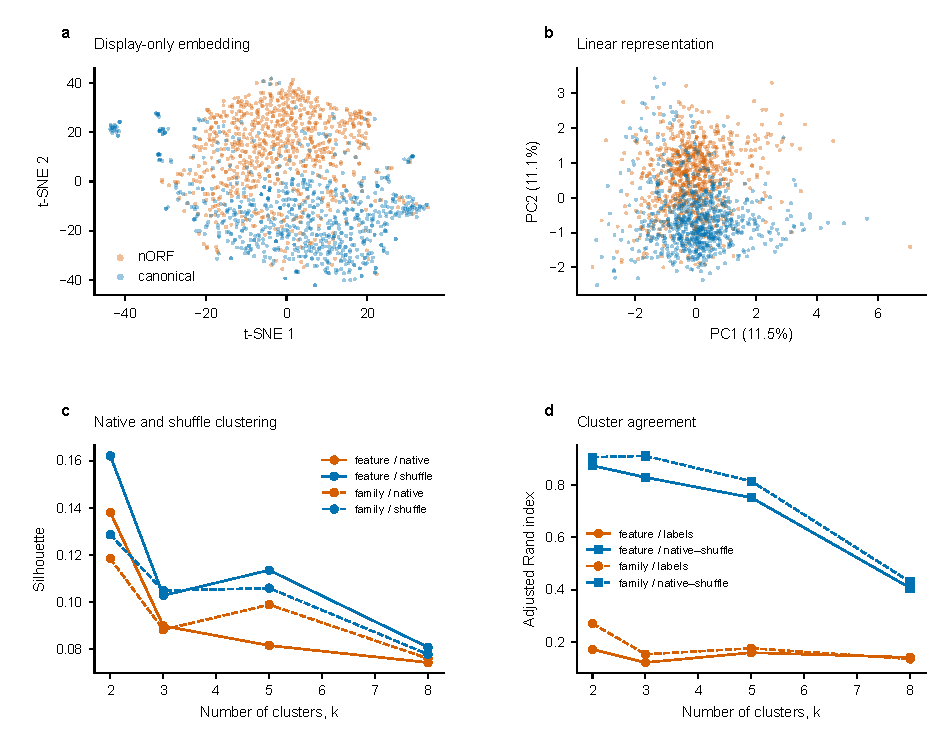
\includegraphics[width=\linewidth]{supplement/FigS1.pdf}
\caption*{\textbf{S1 Fig. Controlled catalogue clustering context.} Controlled catalogue clustering of length-matched canonical and noncanonical
proteins. a,b: illustrative t-SNE/PCA of the same 1,488 matched proteins.
c,d: native/shuffle silhouettes and agreement across $k$ and weighting.
The fixed computational rerun reproduced these controlled maps/memberships;
the original cluster memberships could not be recovered, and functional labels were not tested.
UMAP was not rerun.}
\end{figure}
\clearpage
\section{Detailed benchmark, transfer and exploratory results}
\subsection{Annotation resemblance and reporter accumulation are different targets}
Training on measured reporter outcomes improved prediction substantially. We first define the eligible evaluation cohorts, then compare annotation resemblance, outcome-trained models and the additional information supplied by residue order.

\subsubsection{Dependence controls materially reduce transfer coverage}
The similarity audit covered 4,590 unique native/reference peptides and
2,370,772 eligible alignments. It identified 1,708 primary and 5,319 sensitivity
similarity edges. Across all source types, primary components numbered 3,474,
with a largest component of 254. The 1,072 development constructs occupy 800
groups; the largest contains 156 constructs. Large linked groups are retained,
not split to improve precision (Fig~S2).

\begin{figure}[p]
\centering
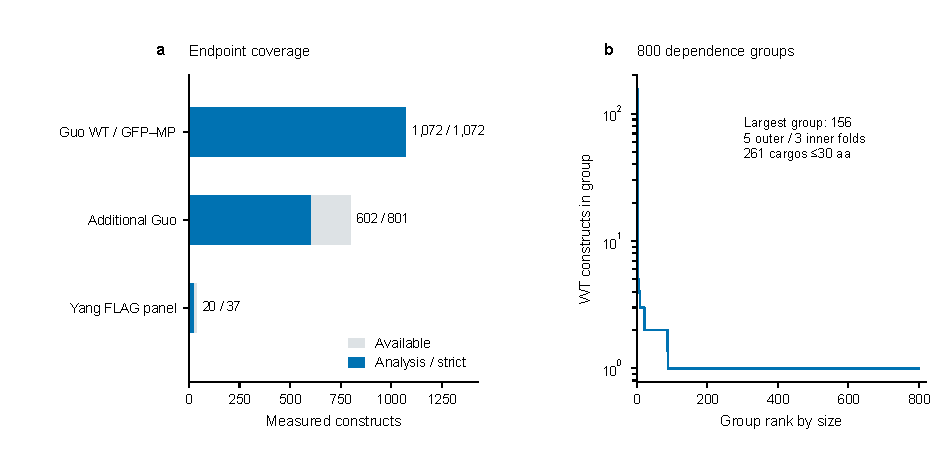
\includegraphics[width=\linewidth]{supplement/FigS2.pdf}
\caption*{\textbf{S2 Fig.} Peptide coverage and validation groups. a: available constructs versus
the development set or strict transfer subset. The 1,072 development cargos
are evaluated by grouped cross-validation, not declared externally independent.
Additional and Yang strict subsets are separated from retrieved Guo groups
as specified. b: development group sizes; the largest contains 156 cargos.
Sequence/gene links can form large components, which are not broken to improve
evaluation.}
\label{fig:coverage}
\end{figure}


Excluding assay-connected components and whole matched reference pairs left
491 balanced annotation pairs from the original 744. No retained pair connects
to a retrieved assay component. Of the 801 additional natural sequences, 602
remain separated from the development groups. Ten Yang peptides exactly match
retrieved Guo natural sequences, and related-sequence/gene links reduce its
strict subset further, from 27 to 20. Current ShortStop-positive counterparts
have no exact matches to the 1,072 development or 801 additional peptides, but
historical and remote-similarity limitations remain.

\subsubsection{Annotation resemblance and reporter ranking diverge}
The independently trained AAC resemblance score correlated negatively with
the native GFP--MP outcome ($\rho=-0.292$, 95\% interval $-0.344$ to $-0.237$).
The three fixed classifier seeds gave $\rho=-0.292$ to $-0.293$, so the negative association did not depend on the chosen seed. ShortStop's mean SAM probability had little monotonic
association ($\rho=-0.018$, interval $-0.077$ to $0.041$; $n=1,057$).
Frozen PAP C30 reached $\rho=0.681$ and its full-sequence secondary transfer
$0.761$ (Fig~1).




Threshold prioritization gives a different result from continuous ranking.
Standard SAM calls ($n=76$) had median reporter score 0.593 versus 0.436 in
other scored cargos, but were longer (median 57 versus 38 aa). A descriptive
rank association after residualizing both continuous score and outcome on
log length and its square was 0.044. There were only 23 consensus-90 and six
consensus-100 calls; their summaries are retained without a strong inference.
These data do not establish that SAM prioritization is useless, or that
PRISM-labelled products lack function. They show that the continuous score
is not a monotonic proxy for this reporter endpoint.

Direct training on the experimental target changed performance substantially
(Table~1). Length alone achieved $\rho=0.207$, AAC model A
$0.747$, and terminal-aware T $0.780$. The strict additional subset preserved
useful composition prediction ($\rho=0.719$). On the same 602 sequences,
ShortStop had $\rho=-0.085$ among its 595 covered peptides, AAC resemblance
$-0.292$, PAP C30 $0.630$, and the released Guo regression $0.737$. The Guo
score is a useful deposited comparator, but released-training disjointness
does not prove blinded external evaluation. No Guo in-sample training estimate
is used in Table~1.
The common-coverage analysis gives the same pattern: on 595 strict additional
cargos, A, T, O and Guo regression achieve $\rho=0.720$, $0.713$, $0.714$
and $0.737$, respectively, versus $-0.292$ for AAC resemblance and $-0.085$
for ShortStop. The common native comparison contains 1,057 cargos.



\subsubsection{Adding residue-order features to T gives small, inconsistent improvements}
The primary O-minus-T rank gain was 0.0040 (95\% interval $-0.0046$ to
$0.0115$), with MAE reduction 0.00077 (interval $-0.00149$ to $0.00332$).
Native order outperformed the three shuffled representations in the primary
point estimates, but its gain over T changed with evaluation context
(Fig~S3). Two additional split seeds gave rank gains of
$-0.00015$ and $0.00517$; 40\% identity grouping gave $0.00594$. In the
opposite orientation O performed worse than T ($\Delta\rho=-0.0102$), as it
did for mutagenesis-library WTs ($-0.0076$). Fixed tree-regression sensitivity
also showed no O advantage over T ($\rho=0.813$ versus $0.814$). Raw order
features gave $\rho=0.785$ in the primary task.

\begin{figure}[p]
\centering
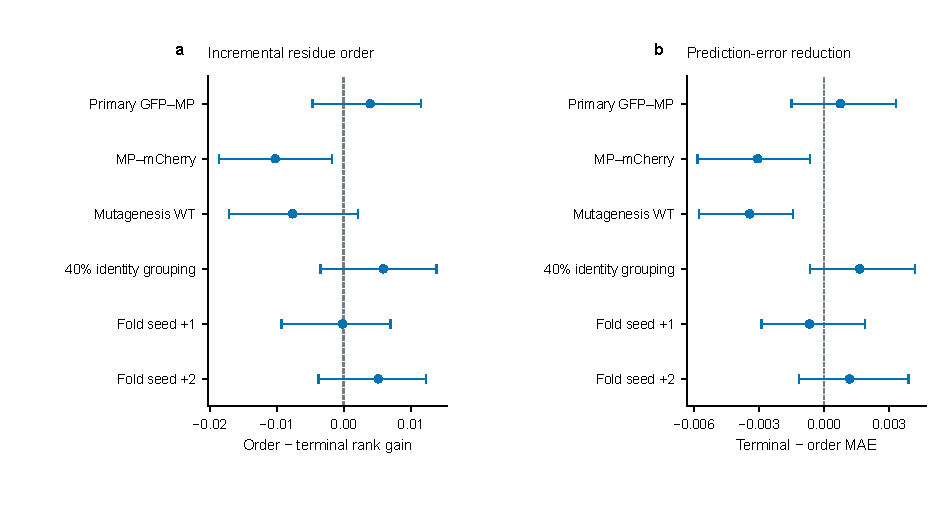
\includegraphics[width=\linewidth]{supplement/FigS3.pdf}
\caption*{\textbf{S3 Fig.} Incremental residue-order prediction relative to the terminal-aware baseline.
Positive values favor O: rank gain is O minus T, error reduction is T minus O.
The 40\% grouping and fold-seed rows use the primary GFP--MP outcomes. Bars
are conditional 95\% group-bootstrap intervals. Orientation and library
changes are endpoint-context sensitivities. Intervals spanning zero do not
constitute formal evidence of equivalence.}
\label{fig:order}
\end{figure}


The median absolute native replicate disagreement was 0.0545; half this is
0.0273, much larger than the primary point MAE reduction, but it is not a
formal minimum useful effect or an equivalence margin. The intervals and sensitivity analyses show that adding these order features gives small and inconsistent improvements. They do not prove that residue order is biologically irrelevant.
All 261 cargos at most 30 aa were retained: their T/O correlations were
0.819/0.817, versus 0.761/0.767 for 811 longer cargos. Complete-replicate,
complexity and ORF-context summaries are supplied without choosing a winning
subgroup. Only ten development peptides met the low-complexity flag, too few
to support a separate conclusion.

\subsubsection{The catalogues remain distinguishable after matching, without establishing functional classes}
Only 9,369 of 27,670 updated nORFs (33.9\%) meet the 31-residue domain of the
default all-family panel, compared with 19,534 of 19,563 canonical representatives.
After exact length matching, AAC discrimination reached AUROC 0.915 versus
0.922 for all 1,440 features. With the GC caliper, corresponding values were
0.864 and 0.882. The previously reported six-feature panel \cite{gounder} attenuated to AUROC 0.661, compared
with 0.950 in its unmatched comparison. These models distinguish the defined populations, but their performance depends strongly on sequence length. They do not classify peptide function.

Broad clustering structure was computationally reproducible under the new
fixed settings (S1 Fig). Family-weighted PCA at $k=2$ had
silhouette about 0.118, catalogue-label adjusted Rand agreement about 0.270,
and native/shuffle agreement about 0.906. Seed agreement was perfect in that
particular setting, with mean 80\% subsampling agreement about 0.964. Finer
clusters, family weights and original-space analyses were more sensitive.
The available historical CSV and default feature code also do not reconcile
with the reported retention count \cite{gounder}. Thus exact historical membership
reproduction remains unresolved, even though the controlled rerun succeeds.

\subsection{Sequence edits and reporter context require separate transfer tests}
A model that ranks unmodified peptides need not predict the effect of an edit or retain its performance in another reporter. We test paired edits, the original source population rules, identical peptides across reporter contexts and a separate expression assay.

\subsubsection{Calibration changes perturbation conclusions}
Native ranking did not translate directly into intervention ranking. Raw PAP
C30 differences correlated with measured Leu-to-Ala effects at $\rho=0.320$
but with extension effects at $-0.005$. Training-WT-only calibration changed
these to 0.374 and 0.124. The secondary full-sequence PAP transfer improved
from raw correlations 0.381/0.057 to calibrated 0.450/0.322 for Leu-to-Ala
and extension, respectively. Thus the exploratory raw extension result cannot
support a blanket claim that the frozen model contains no useful extension
information.

Calibrated full PAP achieved delta MAE 0.1296 and 0.1380, compared with
out-of-group family-mean baselines 0.1485 and 0.1500 (Fig~S4).
WT-trained T achieved 0.1369/0.1668; adding order gave 0.1384/0.1691.
For extension effects, learning that edit family explicitly improved T to
0.1398, whereas opposite-family training gave 0.1594. Opposite-family T
correlations were $-0.122$ for Leu-to-Ala and $0.055$ for extension. These
results distinguish prediction of a native state, learning a perturbation
family and transferring a correction between families.

\begin{figure}[p]
\centering
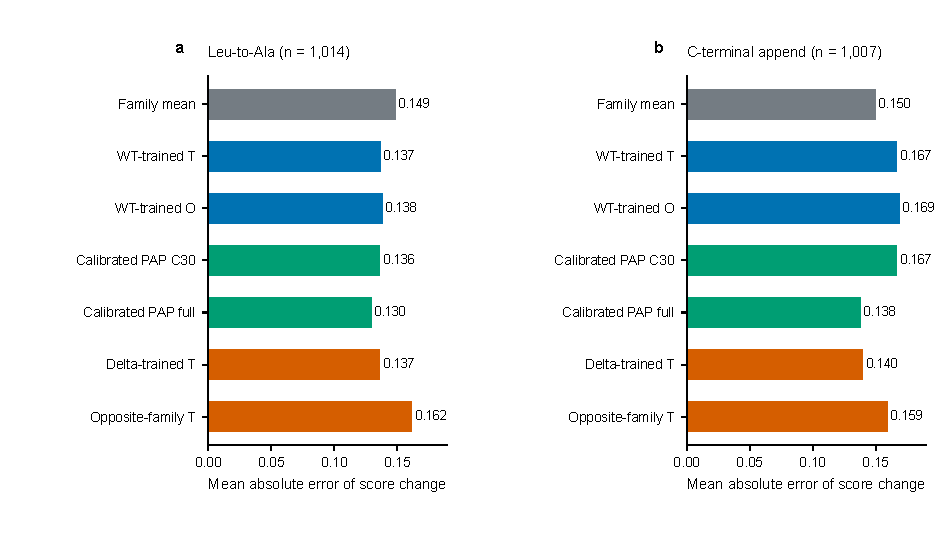
\includegraphics[width=\linewidth]{supplement/FigS4.pdf}
\caption*{\textbf{S4 Fig.} Prediction of within-parent reporter-score changes. All WT-trained
models and isotonic calibrations exclude the evaluated parent group. The
family-mean baseline also excludes that group. Delta-trained models fit
changes from other parents in the same family; opposite-family models use the
other edit family, again excluding test-parent groups. PAP full is a declared
secondary sequence transfer. Raw incompatible score-scale MAE is not plotted.
Ranking, replicate sensitivities and uncertainty are supplied separately.
This figure retains all sequence-valid pairs; Table~S1
and S12 Data add the original-source terminal-Leu restriction.}
\label{fig:mutation}
\end{figure}


AAC resemblance illustrates why score orientation matters: raw delta
correlations were $-0.133$ for Leu-to-Ala and $0.202$ for extension, but WT-fold
calibration yielded $0.074$ and $-0.142$. Its negative native association led
the calibration to reverse direction. Prediction and observed change also
share WT terms; baseline-state coupling and bounded reporter scales can
affect delta correlations. We therefore retain same-library baselines,
calibration directions and replicate-specific analyses, and make no new
mechanistic claim from these associations. The mutation effects themselves
were measured and reported by Guo and colleagues.


\subsubsection{Original-source filtering qualifies the Leu-to-Ala contrast}
On all 1,014 sequence-valid Leu-to-Ala pairs, WT-trained T exceeded A for
mean-change ranking by $\Delta\rho=0.097$ (95\% conditional interval 0.054
to 0.148). Under the original final-two-Leu rule, A and T reached
$\rho=0.315$ and $0.301$ on 798 pairs: their difference was $-0.013$
($-0.032$ to $0.005$; Table~S1). Thus the wider-population
terminal-feature advantage does not persist in this source-defined
substitution population. Append-edit T-minus-A remained positive on both
all 1,007 pairs ($0.393$, 0.321 to 0.470) and the 802 retained pairs
($0.410$, 0.323 to 0.495). Full-PAP source-WT calibration gains on the
retained substitution and append populations were 0.093 (0.030 to 0.142)
and 0.239 (0.186 to 0.301). O-minus-T intervals spanned zero in both.
All 421 omitted family-specific pairs remain available in S12 Data.
These are fixed-prediction, post-hoc population contrasts. They establish
neither a causal effect of the exclusion nor a new terminal confound:
the source authors already specified the rule \cite{guo}.

\begin{table}[H]
\centering\small
\caption{Original-source terminal-Leu sensitivity of mean-change prediction.}
\label{tab:sourcefilter}
\begin{tabular}{llrrr}
\toprule
Edit & Population & Pairs & A & T\\
\midrule
Leu-to-Ala & All valid & 1,014 & 0.262 & 0.359\\
Leu-to-Ala & Source rule & 798 & 0.315 & 0.301\\
Append & All valid & 1,007 & -0.246 & 0.147\\
Append & Source rule & 802 & -0.205 & 0.204\\
\bottomrule
\end{tabular}
\par\smallskip\raggedright\footnotesize
The source rule excludes WTs with Leu at either of the last two positions.
All original fits and predictions are held fixed. A denotes composition;
T adds terminal features. Values are Spearman correlations with same-library
mutant-minus-WT mean scores. S12 Data retains both replicates, omitted strata,
all original predictors and conditional group-bootstrap contrasts.
\end{table}

\subsubsection{Identical peptides show reporter-context dependence}
Guo and colleagues already compared GFP--MP and MP--mCherry reporter
scores in their Supplementary Fig. S6A \cite{guo}. We extend that comparison
to a common three-context cohort and evaluate fitted representation transfer
while holding test peptides and dependence groups fixed.
Matching the same 1,044 peptides removes sequence-cohort composition as the
explanation for differences between the three Guo contexts. Observed
G--M rank agreement was $\rho=0.522$ (95\% group-bootstrap interval
$0.471$ to $0.566$), versus $0.867$ ($0.845$ to $0.889$) for G--U and
$0.496$ ($0.440$ to $0.540$) for M--U (Fig~2).
Within-context biological-replicate correlations were $0.963$ for G
($n=1,043$), $0.986$ for M ($n=1,041$), and $0.877$ for U ($n=1,039$).
These replicate comparisons are descriptive and are not formal prediction
ceilings or an estimate of a causal reporter effect.

Source-trained T retained positive cross-configuration ranking but performed
below target-trained T on identical held-out groups
(Table~2). G-trained T reached $\rho=0.560$ on M,
versus $0.742$ for M-trained T; the paired rank gap was $0.182$
(95\% conditional interval $0.146$ to $0.227$). In the reverse direction,
M-trained T reached $0.566$ on G, versus $0.767$ for G-trained T;
the gap was $0.201$ ($0.163$ to $0.244$). Source-model calibration,
learned from training groups, did not remove these target-scale error gaps:
calibrated-transfer minus target-trained MAE was $0.0490$ for G to M
($0.0408$ to $0.0572$) and $0.0419$ for M to G
($0.0338$ to $0.0492$). Calibration is target-supervised adaptation,
not an independent validation of a frozen predictor.

The composition-only model predicted across the original reporter configurations better than T: A reached $\rho=0.663$ for G to M and $0.648$ for M to G.
Secondary paired contrasts of the saved predictions gave A-minus-T rank
gains of $0.103$ (95\% conditional interval $0.078$ to $0.132$) and
$0.082$ ($0.058$ to $0.104$), respectively. In contrast, T gave higher
within-context point estimates than A for G ($0.767$ versus $0.746$) and
M ($0.742$ versus $0.728$), although the corresponding incremental intervals
included zero. Adding terminal features therefore did not consistently improve prediction across reporter contexts. These feature contrasts were examined after inspecting all A/T
estimates and are explicitly secondary (S8 Data); they do not isolate a
terminal degradation mechanism.



Prediction did not fail in every comparison: performance was better when the reporter stayed the same across libraries. G-trained T reached $\rho=0.691$ on U,
compared with $0.673$ for U-trained T, with calibrated MAE $0.1211$ versus
$0.1305$. In the reverse direction, U-trained T reached $0.737$ on G,
versus $0.767$ for G-trained T. The stronger source-library replicate
agreement is compatible with better source measurements helping prediction,
but does not identify the cause of this asymmetry. The measured-source
bridge required a source assay and achieved target MAE $0.0646$ for G to U,
compared with $0.2078$ for G to M; it is reported separately from sequence
models (S8 Data).

The T rank gap for G to M remained $0.161$ with the 40\% graph and $0.176$
with the second split seed; the reverse gaps were $0.207$ and $0.213$.
Both sensitivity settings also retained the G-to-U source-model advantage.
The complete A-model, calibration, baseline and sensitivity results are
retained in S8 Data. Reporter identity, fusion orientation, construct
architecture and library conditions change jointly, so these observations
cannot identify an isolated tag or terminal-exposure mechanism. They also
do not explain the inverse Yang result or supply an independent replication.

\subsubsection{Independent-study transfer fails to reproduce within-study ranking}
The strict Yang subset contains 20 constructs, of which ten exceed the
published 5\% expression threshold. Primary MP--mCherry-trained T with FLAG
sequence features had $\rho=-0.652$ (95\% interval $-0.888$ to $-0.246$),
and O had $-0.650$. Their AUROCs were 0.16 and 0.15, respectively. Direction
was not inverted after observing validation outcomes. The negative result
persists in the all-37 panel (T $\rho=-0.726$) and is retained as a failed
transfer, rather than hidden by selecting another representation.

Native-only GFP--MP-trained T, a declared context sensitivity, had
$\rho=0.167$ (interval $-0.321$ to $0.616$), whereas its FLAG-aware version
had $-0.303$. FLAG-aware PAP C30 and full transfer had $\rho=-0.124$ and
$0.083$. Native-only full PAP had $0.359$. The result therefore depends strongly on whether the input includes the tag and which reporter orientation supplied the training data (Fig~S5). Neither representation gives convincing evidence of accurate prediction across these assays.

\begin{figure}[p]
\centering
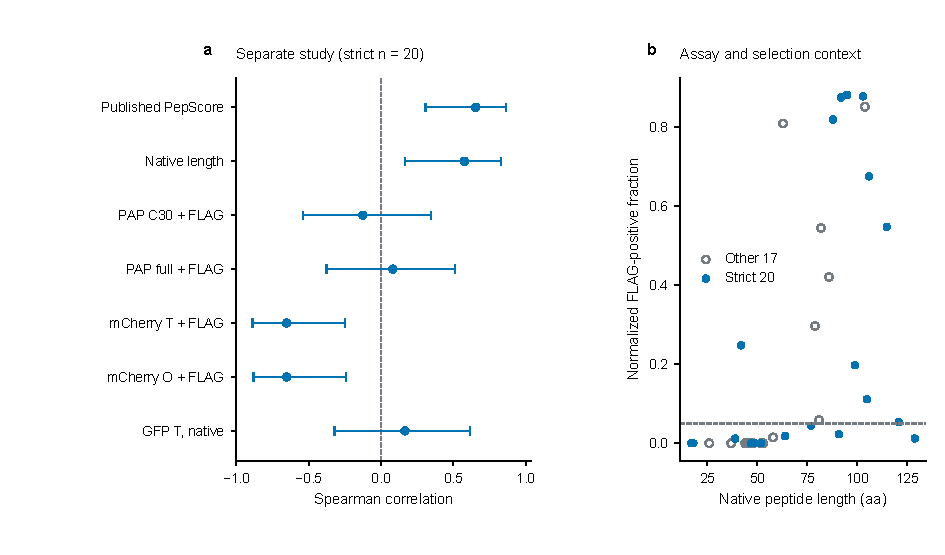
\includegraphics[width=\linewidth]{supplement/FigS5.pdf}
\caption*{\textbf{S5 Fig.} Transfer to a separate FLAG-expression assay. a: strict $n=20$ rank
correlations with conditional group-bootstrap intervals. The primary direct
transfer uses MP--mCherry training and actual FLAG-fusion features. Native-only
GFP--MP transfer is a declared sensitivity, not a post-validation replacement.
PepScore and length refer to the source's mixed panel; this is not an
unbiased method leaderboard. b: all 37 outcomes and native lengths, highlighting
the strict subset. The dashed line is the authors' 5\% expression threshold.
Absolute errors are not compared across assay scales.}
\label{fig:validation}
\end{figure}


Supplied PepScore reached $\rho=0.656$ (interval $0.308$ to $0.865$; AUROC
0.86), while native length alone reached $0.577$ (interval $0.165$ to $0.832$;
AUROC 0.83). The source describes random selection of the 29 uORFs across
PepScores and adds eight high-scoring ORFs of other classes. The combined
panel and validation originate in the PepScore publication.
These estimates therefore do not provide an unbiased external comparison of PepScore with the other methods. A release-wide sequence audit matched ShortStop to 23 constructs
($\rho=-0.058$), including nine of the strict 20 ($\rho=0.268$). This small
covered subset cannot support a strong comparison with methods covering all
20; missing scores were not replaced by zero.

\subsection{Independent transfer depends on the input and comparator}
The independent cohorts test whether favorable within-study results extend to new sequences and interventions. Published predictors, matched sequence inputs and training-exposure audits determine which comparisons support a transfer claim.

\subsubsection{Independent peptide transfer depends on source and decision metric}
Composition models trained only on the source data transferred to the 14,143 eligible canonical
tiles with $\rho=0.816$ for GFP--MP training and $0.817$ for MP--mCherry
training (Table~3). The corresponding T correlations were
$0.812$ and $0.656$. The GFP-trained A-minus-T difference was small and
uncertain: $0.004$ (95\% conditional gene-bootstrap interval $-0.001$ to
$0.010$). The MP--mCherry gap was $0.161$ ($0.149$ to $0.174$).
Thus this target supports a source-specific transfer penalty, not uniform
harm from terminal features. At the stricter similarity threshold, the gaps
were $0.007$ ($0.001$ to $0.012$) and $0.163$ ($0.151$ to $0.176$);
the second source tuning seed retained the pattern (S9 Data).



Feature diagnostics qualify the interpretation (Fig~3).
Removing PAP from T gave external $\rho=0.793$ and $0.648$, respectively.
For GFP-trained heads, C4 gave $0.820$, N4 $0.778$ and I4 $0.793$;
for MP--mCherry training they gave $0.758$, $0.685$ and $0.765$.
Source grouped nested-CV correlations for A/T were $0.747/0.780$ in
GFP--MP and $0.728/0.728$ in MP--mCherry. MP--mCherry N4 reached
$0.763$ in source CV but $0.685$ externally. These diagnostic point
estimates are compatible with context-specific positional information but
do not separate feature complexity from exposure or other construct effects.
Target-study-trained PAP internal/full references reached $0.824/0.862$;
their training provenance prevents a universal external-method ranking.

The secondary selection analysis gave a different GFP-trained comparison.
T selected tiles with a higher mean measured assay score despite its slightly
lower overall rank correlation: A-minus-T selected mean was $-0.0145$
($-0.0211$ to $-0.0073$). For MP--mCherry-trained policies, A selected
higher-scoring tiles: $0.0464$ ($0.0359$ to $0.0564$). Overall correlation alone therefore cannot show which model selects the peptides with the highest measured scores. These are
retrospective policies on canonical peptide reporters, not evidence about
native nORF abundance or biological function.



\subsubsection{Strong published models reduce the apparent advantage of composition-based prediction}
On the same 14,143 native tiles, frozen QCDPred reached $\rho=0.739$ using
complete-window means and $0.800$ using normalized whole-cargo composition
(Fig~4). The latter reduces the A-head advantage to about
$0.016$--$0.017$, with top-decile selected-mean difference intervals spanning
zero (S10 Data). Same-study human25 and PAP references must be distinguished
from these externally trained models. Published PAP CNN1 and CNN7 reached
$0.873$ and $0.877$ on their author-held-out tiles. Thus useful nORF-to-tile
composition transfer does not establish a new composition principle or
superiority over the stronger target-study model.



\subsubsection{Independent paired effects depend on representation and input coverage}
Observed Chu replicate changes correlated at $\rho=0.967$. On the primary
1,743-pair common cohort, GFP-trained A and T predicted mean paired changes
at $\rho=0.617$ and $0.547$. The T-minus-A gap was $-0.070$ (95\% conditional
interval $-0.103$ to $-0.039$). The corresponding mCherry-source values were
$0.622$ and $0.343$ (gap $-0.278$, interval $-0.321$ to $-0.238$).
The poorer performance of these fitted models does not show that terminal information is always harmful: the frozen linear PAP C30 terminal component improved change
ranking by $0.050$ ($0.030$ to $0.068$), whereas its full58 increment was
$0.024$ ($-0.002$ to $0.046$).

Guo-WT-only calibration improved linear full58 PAP from $\rho=0.651$ to
$0.692$, a gain of $0.041$ ($0.027$ to $0.057$; Table~4).
The stronger published neural model narrows that finding: raw full58 CNN1
already reached $0.729$, and calibrated CNN1 reached $0.735$. Its calibration
gain was only $0.006$ ($-0.002$ to $0.014$). CNN7 reached $0.725$ raw and
$0.725$ calibrated, with gain $-0.001$ ($-0.008$ to $0.006$;
Fig~S6). The post-hoc raw-CNN1-minus-calibrated-linear
contrast was $0.037$ ($0.019$ to $0.056$). Calibration improved the linear model, but these results do not show that it generally improves the stronger neural models.



Input coverage had a larger effect than the added neural calibration in this
cohort. Raw CNN1 reached $0.518$ on C30 versus $0.729$ on full58; the post-hoc
gap was $0.211$ ($0.171$ to $0.253$). CNN7 reached $0.524$ versus $0.725$.
This contrast does not isolate a biological cause, and full58 extrapolates
beyond the training length. Both windows, all source contexts, both
replicates, stricter similarity and transcript-match sensitivities remain
reported. Human25 whole-cargo calibration did not improve its primary
change correlation ($0.662$ raw versus $0.655$ calibrated).

\begin{figure}[p]
\centering
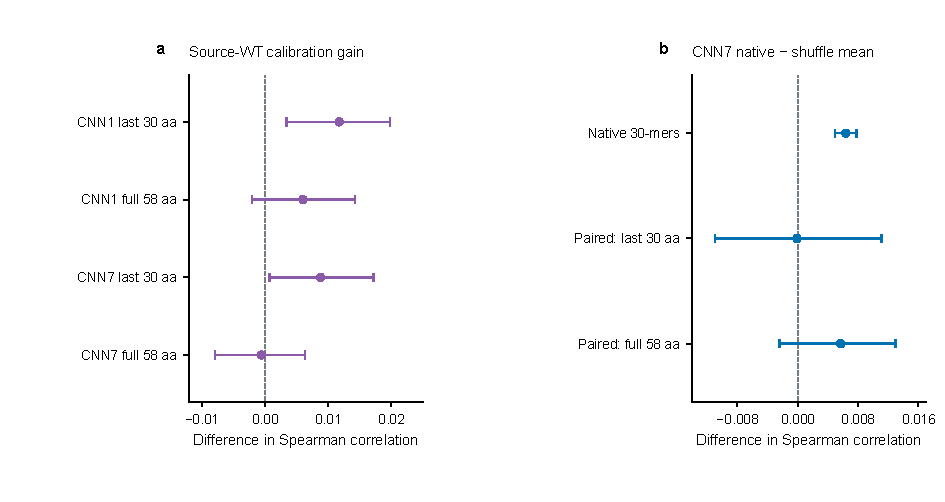
\includegraphics[width=\linewidth]{supplement/FigS6.pdf}
\caption*{\textbf{S6 Fig.} \textbf{Calibration and conditional-order increments depend on the target.}
(a) Calibrated-minus-raw paired-effect correlation for each neural model/input.
Both full58 intervals span zero. (b) CNN7 native-minus-shuffle-mean rank
contrasts preserve composition and the first/final five residues. The native
30-mer result is an author-held-out target-study reference; paired-effect
results use the independent Chu common cohort. Bars are 95\% conditional
group-bootstrap intervals from 1,000 resamples, without multiplicity adjustment. The second shuffle seed and
all raw/calibrated representations are in S10 Data. These are predictive
controls, not measured biological shuffle effects.}
\label{fig:boundaries}
\end{figure}

The conditional order test was positive for native held-out tiles: CNN7
native-minus-shuffle-mean $\Delta\rho=0.0064$ ($0.0050$ to $0.0078$).
Independent paired-effect increments instead had intervals spanning zero:
$-0.0001$ ($-0.0110$ to $0.0111$) for C30 and $0.0057$ ($-0.0024$ to
$0.0129$) for full58. The second shuffle seed gave the same pattern of results.
Separately fitted full58 CNN7 and CNN1 did not establish a change-ranking
advantage (post-hoc difference $-0.0034$, interval $-0.0180$ to $0.0101$).
The model therefore captures a small residue-order signal on native tiles, but we found no clear improvement in predicting independent paired changes.

\subsubsection{Terminal-model comparisons change with exposure and input coverage}
The C23 development-screen audit matched 1,450 WT endpoints and six RT endpoints;
their union covered 1,454 of the 1,743 common-cohort pairs. These pairs cannot
be treated as equally independent terminal-model tests merely because they
passed the separate source/PAP exclusions. Neither endpoint matched in
289 pairs/259 groups; the available-gene-symbol sensitivity retained 97
pairs/88 groups (Table~S2).

\begin{table}[H]
\caption{\textbf{Terminal-model and PAP input-coverage comparisons.}
Entries are correlations with observed RT-minus-WT change on the same pairs
within each row. C23 denotes the final 23 residues; full58 denotes the complete
measured cargo. All-pair terminal results have development-screen exposure.
The 97-pair sensitivity does not certify absence of gene or remote-homology
overlap. All four strata, CNN7/C30 controls and component metrics are in S11 Data.}
\label{tab:terminal}
\centering\small
\begin{tabular}{lrrrr}
\toprule
Exposure stratum & Pairs & C-model & CNN1 C23 & CNN1 full58\\
\midrule
All pairs & 1,743 & 0.500 & 0.479 & 0.729\\
Neither endpoint matched & 289 & 0.537 & 0.521 & 0.761\\
Also no available-symbol match & 97 & 0.669 & 0.651 & 0.779\\
\bottomrule
\end{tabular}
\end{table}

On all pairs, C-model change prediction reached $\rho=0.500$, compared with
$0.479$ for CNN1 on identical C23 inputs and $0.729$ for full58. The
post-hoc same-C23 C-model-minus-CNN1 contrast was $0.021$ (95\% conditional
interval $-0.004$ to $0.042$). On the 289 endpoint-unmatched pairs, these
values were $0.537$, $0.521$ and $0.761$; the same-input contrast was $0.016$
($-0.031$ to $0.064$; Fig~5). All matched-input contrast
intervals span zero. Thus the large contrast against full58 cannot establish
an architecture-only deficit of the terminal model. Equal input coverage
still leaves different training sources and objectives.



C-model correlation rose to $0.669$ in the 97-pair sensitivity, compared with
$0.651$ for CNN1 C23 and $0.779$ for full58. The same-C23 gap was $0.018$
($-0.067$ to $0.117$); the C-model-minus-full58 interval also spanned zero
($-0.110$, interval $-0.269$ to $0.048$). Higher correlations after exclusion
do not demonstrate exposure-caused inflation or absence of exposure effects.
The populations differ, and the smaller sensitivity has wider uncertainty.

\subsection{Exact candidate links define native follow-up experiments}
The results identify candidates for experiments on individual peptides. We match existing reporter edits to full peptide sequences with published interaction and native-evidence annotations. These matches identify candidates to test; they do not show how the edits affect function.

\subsubsection{Candidate interactions remain to be tested after editing}
Of 60 selected Sandmann candidates, 24 had exact full-sequence matches in
natural Guo records; 17 had primary GFP--MP measurements and 32 measured
edit pairs (17 Leu-to-Ala, 15 append). Twenty-eight mean changes were positive
and four negative; all were retained. This selected overlap is not a random
sample or an estimate of functional enrichment. The GAS5 variant shares an
identifier with four Guo records but differs in sequence, so none were
joined. The Sandmann LINC01128 and PVT1 peptides had no exact match.

Three matched candidates carried five source domain/SLiM-associated WT
binding tiles: RP11-620J15.3 (64 residues; CDK5-associated tile), JHDM1D-AS1
(68 residues; two CSNK2A1-associated tiles), and the SLCO5A1 uORF peptide
(55 residues; AURKB- and SRPK2-associated tiles). Their Leu-to-Ala mean
reporter changes were $+0.578$, $+0.120$ and $+0.176$, respectively; append
changes were $+0.126$, $+0.110$ and $+0.121$. All six effects were positive
in both source replicates, and all three WTs passed the source terminal-Leu
rule. These effects are existing Guo measurements, newly linked here to
the exact Sandmann peptide sequences. Global Leu-to-Ala changes residues
within all five WT binding tiles; append retains their sequence. S12 Data
provides every matched and unmatched candidate and residue-level annotation.

A source tagged-overexpression phosphorylation record places JHDM1D-AS1
Ser36 inside its kinase-associated tile region. This provides a separate observation about the candidate. It does not establish endogenous phosphorylation, identify the responsible kinase or show what happens after either edit. No edited binding, native turnover,
peptide-dependent activity or stability--function tradeoff is established.
The canonical SLCO5A1 transporter's activity is not assigned to its uORF.
These candidates can be used to test whether an edit that increases reporter accumulation also preserves interaction. That experiment has not yet been performed.

\subsubsection{Native-source support differs among the three candidates}
Forty-nine of the 60 selected peptides matched the original heart tables
exactly: 36 lncORFs and 13 uORFs. Fifteen had reported positive SRM records.
The heart dataset helped identify candidates for the later panel;
these counts describe coverage, not independent confirmation or functional
enrichment. JHDM1D-AS1 had an in-vitro-translation flag, a shotgun peptide
and three source-positive SRM runs across two hearts. The SRM signature
\texttt{ASMEPPLVAGGLSPR} occupies residues 24--38. The runs had source dot
products 0.7688, 0.7497 and 0.7045 under the original 0.7 threshold
\cite{vanheesch}. These source metrics do not supply a newly calibrated
identification error rate or establish full-product ends or native turnover.

The later community reassessment materially qualifies the shotgun evidence.
The exact JHDM1D-AS1 PSM for \texttt{CRGIQTLENVPPEFPASSK}, scan 21701
in PXD006675, has one recorded curator rating of 1/5, the scheme's
poor-quality category \cite{wacholder}. This does not prove that the peptide
is absent. The study explicitly excluded SRM from reassessment, so this
rating cannot be transferred to the distinct SRM signature or its runs.
The reported targeted evidence still requires claim-specific evaluation.

Forty-five of the 60 candidates matched the 2026 full-sequence catalogue.
RP11-620J15.3, listed there as GIHCG/c12riboseqorf85, and the SLCO5A1
uORF/c8riboseqorf60 each have a source final Tier 2B entry with one
HLA-I peptide \cite{deutsch}. RP11's \texttt{EVCLILKLK} has 10 reported
PSMs but is also mapped to c12riboseqorf86; it cannot uniquely establish
the selected 64-residue product. The uORF's \texttt{TPAPCGTRL} has one
reported PSM. These single-HLA entries are not all manually validated by
the catalogue's more selective annotation workflow. JHDM1D-AS1 has an
exact full-sequence Table 9 row but no entry in the retrieved non-HLA,
HLA or curated-annotation Tables 3, 7 or 12. Missing entries do not establish that translation or function is absent. HLA presentation does not by
itself establish stable accumulation of a full cellular product.

The selected JHDM1D-AS1 peptide is encoded exactly at nucleotides 338--541
of RefSeq NR\_024451.1, with a TAA at 542--544 (1-based). This 2,398-nt
reference differs in overall length from the 951-nt heart assembly.
It is compatible with the reference cited by the 2017 RNA study
\cite{kondo}, without verifying that study's plasmid or peptide expression.
Its SRM signature overlaps both CSNK2A1-associated WT tiles and source
tagged-overexpression Ser36. Leu-to-Ala changes the signature to
\texttt{ASMEPPAVAGGASPR}, whereas append retains it. A WT-signature-only
MS comparison would therefore confound an edited-product measurement
with a changed analyte. Edit-specific standards or a separately validated
common readout are needed before comparing product amounts.

The brain-atlas comparison also distinguishes two peptides sharing the MKKS
name. The selected 63-residue peptide exactly matches micro-MKKS63/Q9HB66,
with a source strong DDA grade and 1,004 unique spectral counts; the separate
50-residue MKKS peptide is listed without MS evidence \cite{brain}.
All 60 candidates were retained, with nine exact Table S2 matches overall.
RP11-620J15.3 is present in the atlas's RiboCode/ShortStop-selected subset
without MS evidence, rather than as an independently confirmed protein.
Neither MKKS peptide has an exact Guo assay match. Micro-MKKS63 could therefore serve as a known native-product control in new experiments. It provides neither an existing WT/edit comparison nor a new functional finding (S15 Data).


\clearpage
\begin{thebibliography}{99}
\bibitem{mudge} Mudge JM et al. Standardized annotation of translated open reading frames. Nature Biotechnology. 2022. \href{https://doi.org/10.1038/s41587-022-01369-0}{doi:10.1038/s41587-022-01369-0}.
\bibitem{chothani} Chothani S et al. An expanded reference catalog of translated open reading frames for biomedical research. Nucleic Acids Research. 2026;54:gkag234. \href{https://doi.org/10.1093/nar/gkag234}{doi:10.1093/nar/gkag234}.
\bibitem{samandi} Samandi S et al. Deep transcriptome annotation enables the discovery and functional characterization of cryptic small proteins. eLife. 2017;6:e27860. \href{https://doi.org/10.7554/eLife.27860}{doi:10.7554/eLife.27860}.
\bibitem{brownmitoribosome} Brown A, Rathore S, Kimanius D, Aibara S, Bai XC, Rorbach J, Amunts A, Ramakrishnan V. Structures of the human mitochondrial ribosome in native states of assembly. Nature Structural and Molecular Biology. 2017;24:866--869. \href{https://doi.org/10.1038/nsmb.3464}{doi:10.1038/nsmb.3464}.
\bibitem{rathoremief} Rathore A et al. MIEF1 Microprotein Regulates Mitochondrial Translation. Biochemistry. 2018;57:5564--5575. \href{https://doi.org/10.1021/acs.biochem.8b00726}{doi:10.1021/acs.biochem.8b00726}.
\bibitem{shepelev} Shepelev NM et al. Translation of numerous upstream open reading frames rather than their products is essential for proliferation of human cells of distinct origin. bioRxiv [Preprint]. 2025 July 7;version 1. \href{https://doi.org/10.1101/2025.07.07.663426}{doi:10.1101/2025.07.07.663426}.
\bibitem{ghosh} Ghosh A et al. Suppressive cancer nonstop extension mutations increase C-terminal hydrophobicity and disrupt evolutionarily conserved amino acid patterns. Nature Communications. 2024;15:9209. \href{https://doi.org/10.1038/s41467-024-52779-4}{doi:10.1038/s41467-024-52779-4}.
\bibitem{hasenjaeger} Hasenj{\"a}ger S, Bologna A, Essen LO, Spadaccini R, Taxis C. C-terminal sequence stability profiling in Saccharomyces cerevisiae reveals protective protein quality control pathways. Journal of Biological Chemistry. 2023;299:105166. \href{https://doi.org/10.1016/j.jbc.2023.105166}{doi:10.1016/j.jbc.2023.105166}.
\bibitem{gounder} Gounder R. The Elusive Dynamic of the Genome: Novel Sequence Patterns, Splicing and Regulation. PhD thesis, University of Cambridge. 2025. Chapter 2 and Appendix A; supplied thesis PDF.
\bibitem{qcdpred} Johansson KE, Mashahreh B, Hartmann-Petersen R, Ravid T, Lindorff-Larsen K. Prediction of quality-control degradation signals in yeast proteins. Journal of Molecular Biology. 2023;435:167915. \href{https://doi.org/10.1016/j.jmb.2022.167915}{doi:10.1016/j.jmb.2022.167915}.
\bibitem{mashahreh} Mashahreh B et al. Conserved degronome features governing quality control associated proteolysis. Nature Communications. 2022;13:7588. \href{https://doi.org/10.1038/s41467-022-35298-y}{doi:10.1038/s41467-022-35298-y}.
\bibitem{zhanginternal} Zhang Z et al. Elucidation of E3 ubiquitin ligase specificity through proteome-wide internal degron mapping. Molecular Cell. 2023;83:3377--3392.e6. \href{https://doi.org/10.1016/j.molcel.2023.08.022}{doi:10.1016/j.molcel.2023.08.022}.
\bibitem{guo} Guo Y et al. Intrinsic bias of the genetic code shapes the folding and stability landscapes of microproteins. Molecular Cell. 2026;86:2173--2190.e11. \href{https://doi.org/10.1016/j.molcel.2026.04.021}{doi:10.1016/j.molcel.2026.04.021}. Data: \href{https://doi.org/10.17632/jjxy3f462r.1}{doi:10.17632/jjxy3f462r.1}.
\bibitem{voutsinos} Voutsinos V et al. A near-complete map of human cytosolic degrons and their relevance for disease. Science Advances. 2026;12:eadz3483. \href{https://doi.org/10.1126/sciadv.adz3483}{doi:10.1126/sciadv.adz3483}.
\bibitem{chu} Chu CY et al. Protein C-terminal variations impact proteostasis. Nature Communications. 2026;17:2288. \href{https://doi.org/10.1038/s41467-026-68979-z}{doi:10.1038/s41467-026-68979-z}.
\bibitem{casola} Casola C, Owoyemi A, Vakirlis N. Degradation determinants are abundant in human noncanonical proteins and minor annotated isoforms. Genome Biology and Evolution. 2026. \href{https://doi.org/10.1093/gbe/evag009}{doi:10.1093/gbe/evag009}.
\bibitem{roginski} Roginski P, Papadopoulos C, Herman S, Baumann A, Grislain A, Lopes A. Impact of GC content on de novo gene birth. Nature Communications. 2026;17:1268. \href{https://doi.org/10.1038/s41467-025-68022-7}{doi:10.1038/s41467-025-68022-7}.
\bibitem{degronopedia} Szulc NA et al. DEGRONOPEDIA: a web server for proteome-wide inspection of degrons. Nucleic Acids Research. 2024. \href{https://doi.org/10.1093/nar/gkae238}{doi:10.1093/nar/gkae238}.
\bibitem{koren} Koren I et al. The eukaryotic proteome is shaped by E3 ubiquitin ligases targeting C-terminal degrons. Cell. 2018;173:1622--1635.e14. \href{https://doi.org/10.1016/j.cell.2018.04.028}{doi:10.1016/j.cell.2018.04.028}.
\bibitem{timms} Timms RT et al. A glycine-specific N-degron pathway mediates the quality control of protein N-myristoylation. Science. 2019;365:eaaw4912. \href{https://doi.org/10.1126/science.aaw4912}{doi:10.1126/science.aaw4912}.
\bibitem{schulze} Schulze TK et al. Supervised learning of protein variant effects across large-scale mutagenesis datasets. Protein Science. 2026. \href{https://doi.org/10.1002/pro.70526}{doi:10.1002/pro.70526}.
\bibitem{mavenn} Tareen A, Kooshkbaghi M, Posfai A, Ireland WT, McCandlish DM, Kinney JB. MAVE-NN: learning genotype-phenotype maps from multiplex assays of variant effect. Genome Biology. 2022;23:98. \href{https://doi.org/10.1186/s13059-022-02661-7}{doi:10.1186/s13059-022-02661-7}.
\bibitem{mochi} Faure AJ, Lehner B. MoCHI: neural networks to fit interpretable models and quantify energies, energetic couplings, epistasis, and allostery from deep mutational scanning data. Genome Biology. 2024;25:303. \href{https://doi.org/10.1186/s13059-024-03444-y}{doi:10.1186/s13059-024-03444-y}.
\bibitem{faureenergetic} Faure AJ, Domingo J, Schmiedel JM, Hidalgo-Carcedo C, Diss G, Lehner B. Mapping the energetic and allosteric landscapes of protein binding domains. Nature. 2022;604:175--183. \href{https://doi.org/10.1038/s41586-022-04586-4}{doi:10.1038/s41586-022-04586-4}.
\bibitem{leblancactivation} LeBlanc CJ et al. Interpretable biophysical neural networks of transcriptional activation domains separate roles of protein abundance and coactivator binding. Cell Systems. 2026;17:101701. \href{https://doi.org/10.1016/j.cels.2026.101701}{doi:10.1016/j.cels.2026.101701}.
\bibitem{gmma} Johansson KE, Lindorff-Larsen K, Winther JR. Global analysis of multi-mutants to improve protein function. Journal of Molecular Biology. 2023;435:168034. \href{https://doi.org/10.1016/j.jmb.2023.168034}{doi:10.1016/j.jmb.2023.168034}.
\bibitem{shortstop} Miller B et al. ShortStop: a machine learning framework for microprotein discovery. BMC Methods. 2025;2:16. \href{https://doi.org/10.1186/s44330-025-00037-4}{doi:10.1186/s44330-025-00037-4}. Precomputed release v1.2.0, 28 October 2026: \url{https://github.com/brendan-miller-salk/ShortStop/releases/tag/v1.2.0}.
\bibitem{yang} Yang H, Li Q, Stroup EK, Wang S, Ji Z. Widespread stable noncanonical peptides identified by integrated analyses of ribosome profiling and ORF features. Nature Communications. 2024;15:1932. \href{https://doi.org/10.1038/s41467-024-46240-9}{doi:10.1038/s41467-024-46240-9}.
\bibitem{trans2ms} He J, Sui J, Chen Q, Hu H, Tan CSH. sORF-Trans2MS: a two-module deep learning framework for sORF translation and MS-supported microprotein prediction. bioRxiv. 2026. Version 1; preprint. \href{https://doi.org/10.64898/2026.09.29.755517}{doi:10.64898/2026.09.29.755517}.
\bibitem{fierro} Fierro-Monti I. Translation uniformity, evolutionary conservation, and peptide properties associate with microprotein mass spectrometry detection. Research Square. 2026. Version 1; preprint. \href{https://doi.org/10.21203/rs.3.rs-9645389/v1}{doi:10.21203/rs.3.rs-9645389/v1}.
\bibitem{xiao} Xiao N, Cao DS, Zhu MF, Xu QS. protr/ProtrWeb: R package and web server for generating various numerical representation schemes of protein sequences. Bioinformatics. 2015;31:1857--1859. \href{https://doi.org/10.1093/bioinformatics/btv042}{doi:10.1093/bioinformatics/btv042}.
\bibitem{hickey} Hickey CM, Breckel C, Zhang M, Theune WC, Hochstrasser M. Protein quality control degron-containing substrates are differentially targeted in the cytoplasm and nucleus by ubiquitin ligases. Genetics. 2021;217:iyaa031. \href{https://doi.org/10.1093/genetics/iyaa031}{doi:10.1093/genetics/iyaa031}. Supplementary Table 5: \href{https://doi.org/10.25386/genetics.13273286}{doi:10.25386/genetics.13273286}.
\bibitem{sandmann} Sandmann CL et al. Evolutionary origins and interactomes of human, young microproteins and small peptides translated from short open reading frames. Molecular Cell. 2023;83:994--1011.e18. \href{https://doi.org/10.1016/j.molcel.2023.01.023}{doi:10.1016/j.molcel.2023.01.023}.
\bibitem{vanheesch} van Heesch S et al. The translational landscape of the human heart. Cell. 2019;178:242--260.e29. \href{https://doi.org/10.1016/j.cell.2019.05.010}{doi:10.1016/j.cell.2019.05.010}.
\bibitem{deutsch} Deutsch EW et al. Expanding the human proteome with microproteins and peptideins. Nature. 2026;654:813--825. \href{https://doi.org/10.1038/s41586-026-10459-x}{doi:10.1038/s41586-026-10459-x}.
\bibitem{wacholder} Wacholder A et al. Community benchmarking and evaluation of human unannotated microprotein detection by mass spectrometry based proteomics. Nature Communications. 2026;17:1241. \href{https://doi.org/10.1038/s41467-025-68002-x}{doi:10.1038/s41467-025-68002-x}.
\bibitem{wacholdercorrection} Wacholder A et al. Author Correction: Community benchmarking and evaluation of human unannotated microprotein detection by mass spectrometry based proteomics. Nature Communications. 2026;17:4882. \href{https://doi.org/10.1038/s41467-026-73431-3}{doi:10.1038/s41467-026-73431-3}.
\bibitem{brain} Miller B et al. A microprotein atlas of the human frontal cortex in Alzheimer's disease. Nature Aging. 2026;6:1979--1997. \href{https://doi.org/10.1038/s43587-026-01207-x}{doi:10.1038/s43587-026-01207-x}. Source repository: \url{https://github.com/brendan-miller-salk/brain-microprotein-atlas}.
\bibitem{schlesinger} Schlesinger D et al. A large-scale sORF screen identifies putative microproteins involved in cancer cell fitness. iScience. 2025;28:111884. \href{https://doi.org/10.1016/j.isci.2025.111884}{doi:10.1016/j.isci.2025.111884}.
\bibitem{kondo} Kondo A et al. Long noncoding RNA JHDM1D-AS1 promotes tumor growth by regulating angiogenesis in response to nutrient starvation. Molecular and Cellular Biology. 2017;37:e00125-17. \href{https://doi.org/10.1128/MCB.00125-17}{doi:10.1128/MCB.00125-17}.
\bibitem{larsen} Larsen FB et al. Comprehensive degron mapping in human transcription factors. Science Advances. 2026;12(45):eaee1766. \href{https://doi.org/10.1126/sciadv.aee1766}{doi:10.1126/sciadv.aee1766}.
\bibitem{salinas2018} Salinas VH, Ranganathan R. Coevolution-based inference of amino acid interactions underlying protein function. eLife. 2018;7:e34300. \href{https://doi.org/10.7554/eLife.34300}{doi:10.7554/eLife.34300}.
\bibitem{architecture} Faure AJ, Mart\'{i}-Aranda A, Hidalgo-Carcedo C, Beltran A, Schmiedel JM, Lehner B. The genetic architecture of protein stability. Nature. 2024;634:995--1003. \href{https://doi.org/10.1038/s41586-024-07966-0}{doi:10.1038/s41586-024-07966-0}.
\bibitem{pdzcomparative} Mart\'{i}-Aranda A, Lehner B. Seven complete comparative maps of allosteric mutations in a protein family. Nature Communications. 2026;17:5487. \href{https://doi.org/10.1038/s41467-026-71005-x}{doi:10.1038/s41467-026-71005-x}.
\bibitem{pdzextensions} Hidalgo-Carcedo C, Faure AJ, Mart\'{i}-Aranda A, Zarin T, Lehner B. Allosteric and energetic remodeling of a PDZ domain by protein domain extensions. Nature Communications. 2026;17:2934. \href{https://doi.org/10.1038/s41467-026-69673-w}{doi:10.1038/s41467-026-69673-w}.
\bibitem{fawzy} Fawzy M, Marsh JA. Understanding the heterogeneous performance of variant effect predictors across human protein-coding genes. Scientific Reports. 2024;14:26114. \href{https://doi.org/10.1038/s41598-024-76202-6}{doi:10.1038/s41598-024-76202-6}.
\bibitem{tripartite} Guharoy M et al. Tripartite degrons confer diversity and specificity on regulated protein degradation in the ubiquitin-proteasome system. Nature Communications. 2016;7:10239. \href{https://doi.org/10.1038/ncomms10239}{doi:10.1038/ncomms10239}.
\bibitem{guharoymasking} Guharoy M, Lazar T, Macossay-Castillo M, Tompa P. Degron masking outlines degronons, co-degrading functional modules in the proteome. Communications Biology. 2022;5:445. \href{https://doi.org/10.1038/s42003-022-03391-z}{doi:10.1038/s42003-022-03391-z}.
\bibitem{middendorf} Middendorf L, Ravi Iyengar B, Eicholt LA. Sequence, Structure, and Functional Space of Drosophila De Novo Proteins. Genome Biology and Evolution. 2024;16(8):evae176. \href{https://doi.org/10.1093/gbe/evae176}{doi:10.1093/gbe/evae176}.
\bibitem{cardiacevolution} Ruiz-Orera J et al. Evolution of translational control and the emergence of genes and open reading frames in human and non-human primate hearts. Nature Cardiovascular Research. 2024;3:1217. \href{https://doi.org/10.1038/s44161-024-00544-7}{doi:10.1038/s44161-024-00544-7}.
\bibitem{vakirlis} Vakirlis N, Vance Z, Duggan KM, McLysaght A. De novo birth of functional microproteins in the human lineage. Cell Reports. 2022;41:111808. \href{https://doi.org/10.1016/j.celrep.2022.111808}{doi:10.1016/j.celrep.2022.111808}.
\bibitem{chenfunctional} Chen J et al. Pervasive functional translation of non-canonical human open reading frames. Science. 2020;367:1140--1146. \href{https://doi.org/10.1126/science.aay0262}{doi:10.1126/science.aay0262}.
\bibitem{prensner} Prensner JR et al. Non-canonical open reading frames encode functional proteins essential for cancer cell survival. Nature Biotechnology. 2021;39:697--704. \href{https://doi.org/10.1038/s41587-020-00806-2}{doi:10.1038/s41587-020-00806-2}.
\bibitem{hofman} Hofman DA et al. Translation of non-canonical open reading frames as a cancer cell survival mechanism in childhood medulloblastoma. Molecular Cell. 2024;84:261--276.e18. \href{https://doi.org/10.1016/j.molcel.2023.12.003}{doi:10.1016/j.molcel.2023.12.003}.
\bibitem{salghetti} Salghetti SE, Muratani M, Wijnen H, Futcher B, Tansey WP. Functional overlap of sequences that activate transcription and signal ubiquitin-mediated proteolysis. Proceedings of the National Academy of Sciences USA. 2000;97:3118--3123. \href{https://doi.org/10.1073/pnas.97.7.3118}{doi:10.1073/pnas.97.7.3118}.
\bibitem{matreyek} Matreyek KA et al. Multiplex assessment of protein variant abundance by massively parallel sequencing. Nature Genetics. 2018;50:874--882. \href{https://doi.org/10.1038/s41588-018-0122-z}{doi:10.1038/s41588-018-0122-z}.
\bibitem{yao} Yao G et al. Long non-coding RNA JHDM1D-AS1 interacts with DHX15 protein to enhance non-small-cell lung cancer growth and metastasis. Molecular Therapy Nucleic Acids. 2019;18:831--840. \href{https://doi.org/10.1016/j.omtn.2019.09.028}{doi:10.1016/j.omtn.2019.09.028}.
\bibitem{malmstrom} Malmstr{\"o}m E et al. The long non-coding antisense RNA JHDM1D-AS1 regulates inflammatory responses in human monocytes. Frontiers in Cellular and Infection Microbiology. 2022;12:934313. \href{https://doi.org/10.3389/fcimb.2022.934313}{doi:10.3389/fcimb.2022.934313}.
\bibitem{liu} Liu C et al. LncRNA RP11-620J15.3 promotes HCC cell proliferation and metastasis by targeting miR-326/GPI to enhance glycolysis. Biology Direct. 2023;18:15. \href{https://doi.org/10.1186/s13062-023-00370-0}{doi:10.1186/s13062-023-00370-0}.
\bibitem{devaux} Devaux A et al. Identification of microprotein-coding intronic polyadenylation isoforms and function in genotoxic anticancer drug response. Genome Biology. 2025;26:366. \href{https://doi.org/10.1186/s13059-025-03829-7}{doi:10.1186/s13059-025-03829-7}.


\end{thebibliography}
\end{document}
